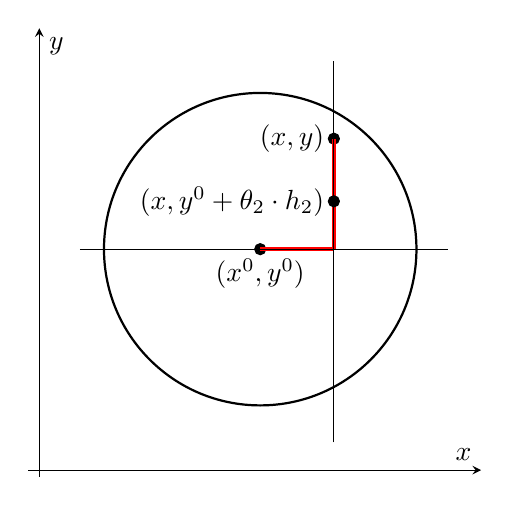
\begin{tikzpicture}[scale=1]
    \begin{axis}[
        axis lines=middle,
        xlabel=$x$, ylabel=$y$,
        xmin=-0.3, xmax=12,
        ymin=-0.175, ymax=12,
        xtick={0},
        ytick={0},
        tick label style={font=\small},
        axis equal image
    ]

    \draw[thick, black](axis cs: 6,6) circle[radius=sqrt(18)];

    \filldraw[black] (axis cs: 6,6) circle (2pt) node[anchor=north]{$(x^{0}, y^{0})$};
    \filldraw[black] (axis cs: 8,9) circle (2pt) node[anchor=east]{$(x, y)$};
    \draw[ultra thick, red] (axis cs: 6,6) -- (axis cs: 8,6);
    \draw[ultra thick, red] (axis cs: 8,6) -- (axis cs: 8,9);
    \draw[thin, black] (axis cs: 8,0.75) -- (axis cs: 8,11.1);
    \draw[thin, black] (axis cs: 1.1,6) -- (axis cs: 11.1,6);
    \filldraw[black] (axis cs: 8,7.3) circle (2pt) node[anchor=east]{$(x, y^{0} + \theta_{2} \cdot h_{2})$};
    
    \end{axis}


\end{tikzpicture}
